\documentclass{beamer}
\usepackage[english,russian]{babel}
\usepackage[utf8]{inputenc}

\usepackage{xskak}
\usepackage{chessboard}

\usepackage{mathtools}
\usepackage{mathrsfs}

\usepackage{amsmath,amssymb,cite,graphicx}
\usepackage{subfigure}
\usepackage{url}
\usepackage{wrapfig}

\usepackage{tikz}
\usetikzlibrary{positioning,shapes,shadows,arrows}
%\usetikzlibrary{arrows.meta}
\usetikzlibrary{graphs}

% Стиль презентации
\usetheme{Frankfurt}
\begin{document}
\title{Эвристический метод поиска неподвижной точки в детерминированной игре с полной информацией} 
\author{Афанасьева А.Е., Афонин С.А.}
%\institute{Московский государственный университет имени М.",В.",Ломоносова}
\institute{Московский государственный университет имени М.",В.",Ломоносова\\
  \vspace{2cm}
}
\date{Москва, 2016} 
% Создание заглавной страницы
\frame{\titlepage} 

% Автоматическая генерация содержания
\frame{\frametitle{Содержание}\tableofcontents}

% Вывести диаграмму с отмеченным ходом
%
\newcommand{\showDiagram}[2]{%
      \chessboard[%
      setpieces={#1},%
      arrow=stealth,%
      linewidth=.25ex,%
      padding=1ex,%
      color=red!55!white,%
      pgfstyle=straightmove,%
      shortenstart=1ex,%
      showmover=false,%
      markmoves={#2},%
      padding=10ex,%
      shortenend=1ex%
      ]%
}


\section{Стратегии в играх с полной информацией}
%{Зачем этим нужно заниматься?}
%\subsection{Введение}
\begin{frame}{Области применения}
Теоретико-игровые модели широко используются для описания различных
практических задач: %в области экономики:
\begin{itemize}
\item планирование, составление расписаний;
\item моделирование военных действий;
\item различные экономические задачи  ??;
\item моделирование принятия решений в психологии.
\end{itemize}
\end{frame}

\begin{frame}{Игры с полной информацией}
Под \emph{играми с полной информацией} понимаются такие игры, в которых каждый из игроков обладает информацией, доступной для принятия решения другими игроками.
 
\bigskip
Доказано существование оптимальной стратегии каждого участника игры для детерминированных игр с полной информацией, но конструктивное его построение 
%- построение полного дерева игры, - 
часто является практически невозможным. 

\bigskip
Пример: шахматы, ...
\end{frame}

\begin{frame}{Поиск оптимальной стратегии}
Методы поиска оптимальной стратегии в заданной позиции (выбор хода) включают:
\begin{itemize}
\item полный перебор путей в дереве игры;
\item перебор с отсечением (альфа-бета процедура);
\item анализ нейронными сетями;
\item эвристические методы.
\end{itemize}
\end{frame}



%\subsection{Как думает человек}
%%\subsection{Как думает человек}
\begin{frame}{Психология принятия решений} 
Игра в шахматы является традиционным предметом изучения психологии принятия решений. Первые работы опубликованы в 1894 году. 

\bigskip
Большой вклад внёсли работы А. де Гроота (1946), Саймона (1982) и другие. Проводились исследования по двум основным направлениям:
\begin{itemize}
\item Восприятие (запоминание позиции)
\item Принятие решения при выборе хода
\end{itemize} 
\end{frame}

\begin{frame}{Восприятие}
\textbf{Эксперимент} 
\begin{itemize}
\item На время $t_1 = 5$с предъявлялась позиция. Через время $t_2 = 30$с предлагалось её восстановить. Анализровался порядок и число правильно восстановленных фигур. 
\end{itemize}
\textbf{Результаты}
\begin{enumerate}
\item На реальных позициях есть различие между экспертами и новичками.
\item Для случайных позиций различия нет.
\item Фигуры рассматриваются логически связанными группами.
\item Некоторые позиции восстанавливаются по ассоциации с другими партиями.
\end{enumerate}
\end{frame}


\begin{frame}{Принятие решения}
\textbf{Эксперимент}
\begin{itemize}
\item Экспертам предъявлялась позиция из реальной партии. Предлагалось выбрать наилучший ход. Производить рассуждения требовалось вслух.   
\end{itemize}
\textbf{Результаты}
\begin{enumerate}
\item Рассматривается небольшое число ходов-кандидатов.
\item Небольшая глубина анализа (до 5 ходов) вне зависимости от мастерства.
\item Дерево анализа содержит $20-80$ узлов. 
\item Частые возвращения назад: анализ хода или эпизода часто повторяется.  
\end{enumerate}
\end{frame}

\begin{frame}{Теория прогрессивного углубления}
По результатам проведенных исследований де Гроотом были выделены основные фазы мышления шахматиста\footnotemark{}
\begin{itemize}
\item ориентировка (выделение группы ключевых фигур);
\item разведка (пробы нескольких ходов);
\item обработка (систематический глубокий просчёт вариантов);
\item доказательство (проверка надёжности результата).
\end{itemize}
\footnotetext{de Groot A.D., 1946, 2008. Thought and Choice in Chess,  Amsterdam University Press // Amsterdam Academic Archive.}
\end{frame}

%\AtBeginSubsection[]
%  {
%     \begin{frame}<beamer>
%     \frametitle{Содержание}
%     \tableofcontents[currentsubsection]
%     \end{frame}
%  }

%\subsection{Как играют современные программы}
%%\subsection{Существующие подходы}

\begin{frame}{Полный перебор}
В 1913 году в работе Цермело\footnotemark{} было доказано существование оптимальной стратегии игры с полной информацией.
Подход состоит в построении полного дерева игры.
\begin{figure}
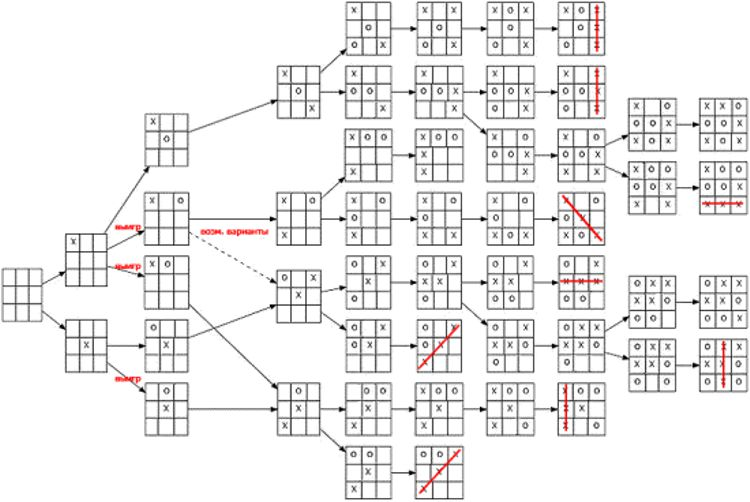
\includegraphics[scale=0.3]{./pictures/xoxo.jpg}
\end{figure}
\footnotetext{Е. Zermelо, Obereine Anwendung der Mengenlehre attfdie Theorie des Schachspiels (Cambridge, 1913)}
%Zermelo E. Über eine Anwendung der Mengenlehre auf die Theorie des Schachspiels //Proceedings of the fifth international congress of mathematicians. – II, Cambridge UP, Cambridge, 1913. – Т. 2. – С. 501-504.
\end{frame}

%\begin{frame}{Полное дерево игры}
%\begin{figure}
%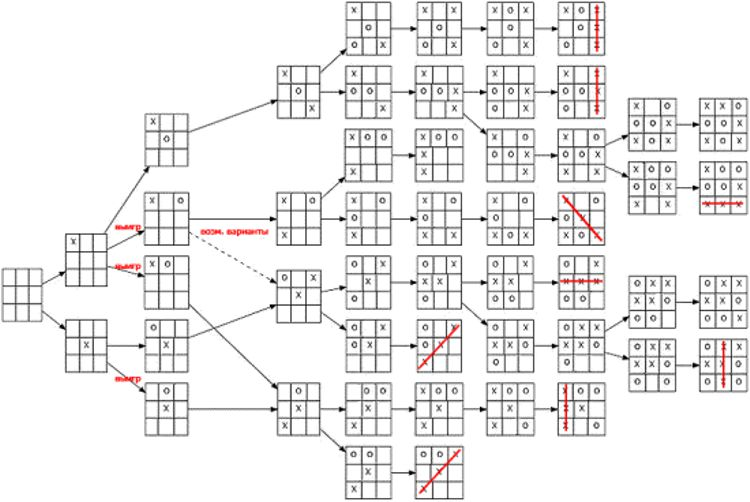
\includegraphics[scale=0.5]{./pictures/xoxo.jpg}
%\end{figure}
%\end{frame}

\begin{frame}{Особенности переборного подхода}
\begin{itemize}
\item После $m$ ходов дерево игры содержит порядка $d^m$ листов, где $d$ -- среднее количество возможных ходов в позиции.
\item Для крестиков-ноликов $d \approx 5$, для шахмат $d \approx 60$, для~го~$d \approx 400$. 
\item Построение требует большой вычислительной мощности.
\item Включает в себя множество очевидно бессмысленных ходов.
\item Проводится сокращение дерева с помощью различных эвристических методов (minimax, alpha-beta и другие).
\item У современных программ, с учетом отсечений, осуществляется перебор $100.000$ позиций в секунду. (<<Rybka>>)
\end{itemize}
\end{frame}

%ГУГЛ!
\begin{frame}{Нейронные сети}
Игровые задачи часто используются как способ тестирования и проверки эффективности применения алгоритмов автоматического обучения\footnotemark{}. 
\begin{itemize}
\item Лучший ход рассматривается как функция от текущего расположения фигур на доске.
\item Требует больших объемов обучающих данных.
\item Возможно самообучение.
\item Достигнуты выдающиеся результаты: 13-ти слойная нейронная сеть
  одержала победу 4:1 над одним из сильнейших игроков мира в го Ли
  Седолем.
\item Объяснить выбор конкретного хода нельзя.
\end{itemize}
\footnotetext{Silver D. et al. Mastering the game of Go with deep neural networks and tree search //Nature. – 2016. – Т. 529. – №. 7587. – С. 484-489.}
\end{frame}


%\subsection{Сравнение}
%
%\subsection{Сравнение}
\begin{frame}{И всё-таки зачем}
\begin{figure}
%Шахматные турниры...
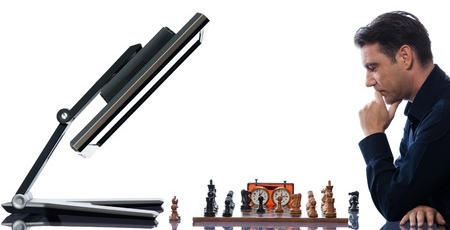
\includegraphics[scale=0.55]{./pictures/vs.png}
\end{figure}
\begin{columns}
\column{0.5\textwidth}
\begin{itemize}
\item Позиции анализируются независимо
\item Большой объем обрабатываемых данных
\item Сложно объяснить принципы выбора хода
\end{itemize}
\column{0.5\textwidth}
\begin{itemize}
\item Блочное восприятие
\item Ограниченный перебор
\item Прогрессивное углубление
\item Долгосрочное планирование
\end{itemize}
\end{columns}

\smallskip
Нет реализаций, учитывающих психологические аспекты.
\end{frame}

\endinput

\begin{frame}{Зачем этим нужно заниматься?} 
\begin{itemize}
\item Шахматы, как игра с полной информацией, сводится к решению задачи комбинаторной оптимизации.
\item Человек способен эффективно решать подобные задачи неформальным способом.
\item Существующие игровые программы основываются на иных методах решения.
\item В точности определить подход, используемый человеком, на данный момент не удалось.
\end{itemize}
\end{frame}


\begin{frame}{Сравнение и почему ничего не подходит}
\begin{itemize}
\item  практические результаты достигнутые программами значительно превосходят человеческие. Обыграли человека во всех играх (в т.ч. Го)
\item Анализ большого количества данных (статистических или в ходе построения дерева)
\item Не учитываются психологические аспекты.
\item Отсутствует стратегическое дальносрочное планирование.
\item Процесс мышления человека смоделировать не удалось.
\end{itemize}
\end{frame} 


\AtBeginSection[]
  {
     \begin{frame}<beamer>
     \frametitle{Содержание}
     \tableofcontents[currentsection]
     \end{frame}
  }
  
%\subsection{Метод М.М. Ботвинника}
%%\subsection{Подход М.М.Ботвинника}
\begin{frame}{Подход М.М.Ботвинника}
Ботвинник предлагал анализировать расположение фигур на статической доске. Для этого необходимо: 
\begin{itemize}
\item определить локальные цели для данной позиции;
\item наметить план достижения цели;
\item проверить осуществимость плана;
\item объединить планы в единое представлене о позиции;
\item определить оптимальную последовательность действий.
\end{itemize}
Данный подход рассматривался, как средство решения широкого класса комбинаторно-оптимизационных задач.
\end{frame}

\subsection{Основные понятия}
\begin{frame}{Основные понятия}
\begin{description}
\item[Траектория] последовательность полей движения фигуры на пустой доске
\item[Горизонт] максимальная длина рассматриваемых траекторий
\item[Цель] фигуры противника или поля
\item[Подцепочка] действия, направленные на достижение цели
\item[Цепочка] совокупность действий, направленных на достижение цели
\item[Вилочность] совпадение частей цепочек
\item[Оценка фигуры] числовая характеристика <<полезности>> фигуры
\item[Время успевания] допустимое число ходов для защиты от атаки противника
\end{description}
\end{frame}

\begin{frame}{Основные понятия: пример цепочки}
\begin{columns}
\column{0.5\textwidth}
\begin{figure}[t]
  \centering
  \subfigure[1.]{%
    \scalebox{0.8}{%
      \setchessboard{showmover=true}%
      \chessboard[setpieces={Pa5, Na7, bh3},%
      arrow=stealth,%
      linewidth=.25ex,%
      padding=1ex,%
      color=red!55!white,%
      pgfstyle=straightmove,%
      shortenstart=1ex,%
      showmover=false,%
      markmoves={a5-a8},%
      padding=10ex,%
      shortenend=1ex%
      %, markmoves={f3-g3,g3-h4}%
      ]%
    }%
  }
\end{figure}
\column{0.5\textwidth}
\textbf{Цель} - достижение пешкой поля a8 \\
\textbf{Траектория} - a5-a6-a7-a8. \\
\pause
\textbf{Подцепочка-1} - освобождение траектории a7-b5, a7-c6, a7-c8. \\
\pause
\textbf{Подцепочка-1} - защита противника h3-g2-(a8), h3-f1-(a6) \\
\pause
\textbf{Подцепочка-2} - поддержка a7-b5-c7-(a8, a6), a7-c8-b6-(a8)
\end{columns}
\end{frame}


\subsection{Примеры и обобщения}
\begin{frame}{Примеры на модельных задачах} %без королей
Позиция, \\
анализ, \\ 
пример цепи (цель). 
\end{frame}

\begin{frame}{Обобщение}
Лингвистическая геометрия \\
Экономика
\end{frame}

\begin{frame}{Проблемы} % +диаграммы на каждый пункт с примерами 
Динамический горизонт событий \\
Динамическая оценка фигур и цепей \\
Связь между цепочками \\
Траектории с подвижной целью \\
Оптимальность цепи
%НЕТ ФОРМАЛИЗАЦИИ!! \\
\end{frame}

\begin{frame}{Метод М.М. Ботвинника: понятие цепочки}
\centering
\begin{tabular}{l}
  {\hspace{-0.3cm}\scalebox{0.6}{\showDiagram{Ka1, Pa5, Na7, kh8, bh3}{}}}
  \hfill%
  \begin{tikzpicture}[scale=0.56]
    \begin{scope}[every node/.style={fill=white,circle,thick,draw,inner sep=0.5pt,font={\fontsize{7.20}{7.44}\selectfont}}]
      \node [label=above:{\setboardfontsize{0.4cm}{\textcolor{black}{\WhitePawnOnWhite}}}] (A5) at (0,0) {a5};
      \node (A6) at (2,0) {a6};
      \node (A7) at (4,0) {a7};
      \node (A8) at (6,0) {a8};
      \node [label=left:{\setboardfontsize{0.4cm}{\textcolor{black}{\WhiteKnightOnWhite}}}] (NA7) at (1,2.5) {a7};
      \node (B5) at (4,2.5) {b5};
      \node (C6) at (3,1.5) {c6};
      \node (C7) at (7,2.5) {c7};
      \node (C8) at (1.5,1.3) {c8};
      \node [label={45:{\setboardfontsize{0.4cm}{\textcolor{black}{\BlackBishopOnWhite}}}}] (H3) at (3,-3) {h3};
      \node (G2) at (6,-3) {g2};
      \node (F1) at (0.5,-1.7) {f1};
      \node (BC8) at (1.8,-1.7) {c8};
    \end{scope}

    \begin{scope}[>={stealth},
      % every node/.style={fill=white,circle},
      every edge/.style={draw=red,very thick}]
      % подцепочка 0
      \path [->] (A5) edge node [text width=0.5cm,midway,above] {} (A6); %  {B} 
      \path [->] (A6) edge (A7);
      \path [->] (A7) edge (A8);
      % Защита
      \path [->] (H3) edge[draw=black] (G2);
      \path [->] (G2) edge[gray, draw=gray, dashed] (A8);
      \path [->] (H3) edge[draw=black] (F1);
      \path [->] (F1) edge[gray, draw=gray, dashed] (A6);
      \path [->] (H3) edge[draw=black] (BC8);
      \path [->] (BC8) edge[gray, draw=gray, dashed] (A6);

      % Отступление 
      \path [->] (NA7) edge[draw=black] (B5);
      \path [->] (NA7) edge[draw=black] (C6);
      \path [->] (NA7) edge[draw=black] (C8);
      \path [->] (B5) edge[draw=black] (C7);
      \path [->] (B5) edge[gray, draw=gray, dashed] node [rotate=-90,above,yshift=0.15cm] {\textcolor{black}{$\stackrel{\text{\tiny подцепочка}}{\text{\tiny к полю}}$}} (A7);
      \path [->] (C7) edge[gray, draw=gray, dashed, bend left] (G2);
      \path [->] (C7) edge[gray, draw=gray, dotted] node [rotate=67,above,yshift=0.1cm] {\textcolor{black}{\tiny контроль}} (A8);
      % \path [->] (B) edge[bend right=60] node {$1$} (E); 
      \path [->] (C6) edge[draw=black, opacity=0.3, dotted, bend right] node [rotate=0,above,yshift=0.1cm] {\textcolor{black}{\tiny блокада g2-a8}} (G2);
    \end{scope}
  \end{tikzpicture}
\end{tabular}

Цепочка порождается последовательностью ходов (траекторией движения фигуры), а так же вспомогательными действиями, связанными с некоторыми
полями основной траектории. Каждая цепочка описывает возможное развитие игры в
случае выбора игроком данной цели.
\end{frame}


\begin{frame}
\frametitle{\only<1,3>{Pro et contra}
			\only<2>{Когнитивные процессы}}
\only<1,3>{
Преимущества подхода:
\begin{itemize}
\item строится план, а не один ход;
\item может использоваться для решения не только шахматных задач;
%, например, планирования.
\item соответствует особенностям мышления человека.
\end{itemize}
}

\only<2>{
%В данной работе ставится задача моделирования 
%Процесс поиска оптимальной стратегии, согласуется с данными психологических исследований шахматистов (де~Гроот, Саймон и др.), согласно которым шахматистам свойственно:
Психологические исследования шахматистов (де~Гроот, Саймон и др.) выявили следующие особенности мышления:
\begin{itemize}
\item восприятие позиции группами логически связанных фигур;
\item ограниченный перебор ($\approx 50-70$ позиций);
\item прогрессивное углубление;
\item долгосрочное планирование;
\item использование аналогий (типовые позиции).
\end{itemize} 
}

\only<3>{
Почему не было реализовано:
\begin{itemize}
\item недостаточные вычислительные мощности; %мегабайты памяти на тысячи цепочек.
\item отсутствие строгой формализации задачи;
\item \alert{сложнее}, чем построение дерева игры;
\item снижение интереса к задаче моделирования шахматиста, в связи с превосходством переборных алгоритмов над человеком.
\end{itemize}}
%При построении дерева достаточно иметь функцию оценки позиции и использовать минимакс. 
%Метод Ботвинника существенно сложнее, чем построение дерева игры.
\end{frame}


%здесь начинается своё
\section{Поиск неподвижной точки}

%Что хотим найти
\begin{frame}{Оптимальное представление позиции}
%Как неподвижная точка...
Представление позиции~--- набор цепочек, т.е. цели и способы их достижения, на котором задана функция оценки.

\smallskip
\smallskip
Рассмотрим граф представлений.

\begin{wrapfigure}[6]{l}{0.56\linewidth} 
%\center
\vspace{-3ex}
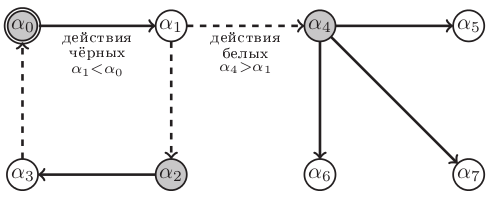
\includegraphics[width=0.56\textwidth]{graph_example}
%\caption{Схема графа представлений.}
\end{wrapfigure}

Дуги отражают изменения поднаборов цепочек определенного цвета, улучшающие оценку с точки зрения соответствующего игрока.

\smallskip
\smallskip
Неподвижная точка --- оптимальное представление позиции ~---
это набор цепочек, изменение которого невыгодно ни
одной из сторон.

%Перебор не ходов, а <<планов>>.
\end{frame}

%Почему сложно
\begin{frame}{Трудности реализации метода}
%Заметим, что оценка цепочки зависит от стоимости фигур, которые участвуют при реализации данной цепочки. В то же время стоимость фигуры зависит от оценки цепочек, в которых она задействована. Изменение стоимости фигуры может повлечь за собой изменение структуры цепочек или даже их исчезновение.

%Проблемы с примерами:
Выделим несколько основных сложностей, возникающих при решении задачи построения оптимального представления позиции.
\begin{enumerate}
\item Большое количество цепочек и подцепочек.
% --- процедура доопределения. 
% 2^6 для белого короля из этюда Рети
\item Связи между различными цепочками (завлечение, двойной удар, отвлечение).
%(дерево фигур), ищем вилочность.

\item Нельзя ограничить глубину построения цепочек (время успевания).
%этюд Рети

\item Зависимость между оценкой фигуры и оценкой цепочки или представлением позиции. 
%(Пример пропадающих или изменяющих структуру цепочек).

%4. траектории нулевой длины и область допустимого перемещения


%6. позиционно фигура может стоить меньше, чем базовая стоимость.

%7. выделение перспективных цепочек в представление на след. итерации (шах и мат?), изменение оценки при доопределении (может только уменьшиться)

%8. оценка таргетов, на который можно напасть множеством способов ?

\end{enumerate}
\end{frame}


\begin{frame}
\frametitle{\only<1> {Этюд Р.~Рети (1921): взаимосвязь цепочек}}
\begin{columns}
\column{0.5\textwidth}
\vspace{-5ex}
\begin{figure}[t]
  %\only<1,3,5>{\scalebox{0.8}{\showDiagram{Kh8, Pc6, ka6, ph5}{}}}
  %\only<2>{\scalebox{0.8}{\showDiagram{Kh8, Pc7, ka6, ph5}{a6-b7}}}
  %\only<4>{\scalebox{0.8}{\showDiagram{Kh7, Pc6, ka6, ph5}{h5-h4}}}
  %\only<6>{\scalebox{0.8}{\showDiagram{Ke7, Pc6, ka6, ph5}{}}}
  %\only<7>{\scalebox{0.8}{\showDiagram{Ke7, Pc7, ka6, ph5}{}}}
  %\only<8>{\scalebox{0.8}{\showDiagram{Ke7, Pc7, kb7, ph5}{}}}
  %\only<9>{\scalebox{0.8}{\showDiagram{Kd7, Pc7, kb7, ph5}{}}}
  \only<1>{\scalebox{0.8}{\showDiagram{Kh8, Pc6, ka6, ph5}{h8-e5, f6-e7, e5-d6, e5-h2}}}
\end{figure}
%\only<1-9>{Ход белых. Ничья.}
\column{0.5\textwidth}
%\only<2>{Провести свою пешку в ферзи не удаётся, так как король черных её легко догоняет.}
%\only<4>{Догнать чёрную пешку не получается. Она убегает.}
%\only<5>{Что же тогда делать?}
%\only<6-9>{Если король белых был бы на поле e7, то можно было бы пойти \alert<7>{1. c7} \alert<8>{Kb7} \alert<9>{2. Kd7} и 3. c8Q}
\only<1>{{Решение получаем объединением двух идей (двух цепочек).\\
 \smallskip Первая~--- Крh8-g7-f6-e7 (подцепочка-1 для c6-c7-c8Ф).\\
\smallskip Вторая~--- Крh8-g7-f6-e5-f4-g3-h2 (<<защитная>> подцепочка-1 для h5-h4-h3-h2-h1Ф)}}
\end{columns}
\only<1>{Траекторий h8-h2 --- $2^5$. \\
Наличие общей части позволяет выиграть необходимое время.}
\end{frame}

%Как хотим делать 
\begin{frame}{Метод поиска неподвижной точки}
%Найти оптимальное представление позиции методом перебора всех вариантов представлений практически невозможно, поэтому предлагается использовать итерационный алгоритм поиска приближения $\Gamma^*$.
\begin{enumerate}
\item Строим все \emph{полные цепочки}. % на статической доске
\item Составляем \emph{деревья фигур}, содержащие все их траектории и цепочки. Дерево фигуры позволяет выявить траектории движения фигуры, общие для нескольких цепочек.
\item Оцениваем каждую вершину дерева фигуры: изменение положения фигуры может сделать возможным или невозможным ее участие в некоторых цепочках.
\item Выделяем наиболее быстрые и выгодные цепочки, и доопределяем их, выбирая подцепочки, <<оптимальные>> согласно деревьям фигур. Обозначим полученный набор $\Gamma$.
\item Строим граф представлений исходящий из вершины $\Gamma$.
\item Методом минимакса на графах находим $\Gamma^*$.
%\item Переоцениваем фигуры и ищем приближение $\Gamma^*$ как \emph{неподвижную точку} в оценке цепочка-фигура.
\end{enumerate}
\end{frame}

%\begin{frame}{Упрощения задачи}

%Представление позиции строится при статичном положении фигур, поэтому далее необходимо выбрать по $\Gamma^*$ ходы-кандидаты и проверить их перебором на виртуальной доске.

%Рассматривается статическая доска, целевые фигуры не ходят (будет потом), пока горизонт статический (зависит от ситуации на доске, этапа игры и рассматриваемой фигуры), не ищем шах и мат?
%не решаем задачу поиска первого хода в позиции.
%\end{frame}

%\subsection{Понятие оптимальности}
%\begin{frame}{Оценочная функция}
Для вычисления оценочной функции цепочки необходимы: \\
$ep_{chain} \left(n\right) \in 2^{\mathtt{Pieces}}$ --- множество фигур, участвующих в размене на $n$-ом поле траектории. \\
$value\left(p\right) \in \mathbb{Z}$ --- стоимость фигуры, белые фигуры имеют положительную оценку, черные -- отрицательную.\\ 
$len_{chain}\left(traj\right) \in \mathbb{N}^+$ --- длина траектории. \\
Определим оценочную функцию $\varphi \colon \mathtt{Chains} \to \mathbb{N}$:
$$
 \varphi \left( ch \right) = \sum_{k \in \left[0, l\right]} \sum_{ p \in ep\left(k\right)} value\left(p\right) + \sum_{sch \in sa\left(k, traj\right)} \varphi\left(sch\right)
$$
Согласно полученной оценке, построим граф, узлами которого являются оцененные цепочки, имеющие одинаковую изначальную структуру - подцепочку-0.
\end{frame}

\begin{frame}{Граф цепочек}
 Если две цепочки $\left(\Gamma_{0, 0}, \alpha_0\right)$ и $\left(\Gamma_{0, 1}, \alpha_1\right)$ таковы, что $\alpha_0 > \alpha_1$, то проводится ребро черного цвета. Это означает, что черные могут улучшить оценку в свою пользу. 
%\begin{tabular}{ll}
\begin{tikzpicture}
\begin{scope}[every node/.style={circle,thick,draw}]
    \node (00) at (0,0) {$\Gamma_{0, 0}, \alpha_0$};
    \node (01) at (3,0) {$\Gamma_{0, 1}, \alpha_1$};
    \node (21) at (6,0) {$\Gamma_{2, 1}, \alpha_4$};
    \node (11) at (3,-3) {$\Gamma_{1, 1}, \alpha_2$};
    \node (10) at (0,-3) {$\Gamma_{1, 0}, \alpha_3$};
    \node (22) at (9,0) {$\Gamma_{2, 2}, \alpha_5$};
    \node (23) at (6,-3) {$\Gamma_{2, 3}, \alpha_6$};
    \node (24) at (9,-3) {$\Gamma_{2, 4}, \alpha_7$};
\end{scope}
\begin{scope}[%>={Stealth[black]},
              every node/.style={fill=white,circle},
              every edge/.style={draw=black,very thick}]
    % подцепочка 0
    \path [->] (00) edge (01);
    \path [->] (11) edge (10);
    \path [->] (21) edge (22);
    \path [->] (21) edge (23);
    \path [->] (21) edge (24);
    \path [->] (01) edge[dashed] (21);
    \path [->] (01) edge[dashed] (11);
    \path [->] (10) edge[dashed] (00);
\end{scope}
\end{tikzpicture}
%&\end{tabular}
\end{frame}

\begin{frame}{Оптимальная цепочка}
Выбор цепочки с нашей стороны определяется максимальным значением оценочной функции, в то время как противник, наоборот, стремится реализовать цепочку, которая её минимизирует. \\
То есть, противник выбирает цепочку той же структуры нашего цвета, заменяя в ней подцепочки своего цвета, чтобы максимально уменьшить оценку. \\
В случае цикла, \textbf{оптимальным} считается тот узел, в котором при наилучшем выборе противника, мы имеем возможность улучшить оценку. \\
При линейной структуре \textbf{оптимальна} листовая вершина с максимальной оценкой.
\end{frame}

\begin{frame}{Трудности нахождения оптимальной цепочки} %граф, содержащий всё.
Основная трудность заключается в построении графа цепочек, так как при построении необходимо включать в него всевозможные цепочки. \\
Вместо полного перебора вариантов, хотелось бы иметь структуру, достраивающую подцепи динамически, если возникает такая необходимость.\\
Так же оценка фигур не является фиксированным числом, а зависит от цепочек, в которых она участвует. \\
Одна и та же фигура в одной цепочке может выполнять несколько функций, то есть, участвовать в нескольких подцепочках. В зависимости от временных рамок, её поведение так же может различаться. 
%Непонятно об оценке фигур и связях между фигурами в цепочках (в двух подцепях по-разному, можно ли ходить вдоль траектории, или нельзя).
\end{frame}

\endinput
\begin{frame}{Результаты}
{{$$\begin{cases}
\alpha_0 < \alpha_1 \\
\alpha_1 > \alpha_2 \\
\alpha_2 < \alpha_3 \\
\alpha_3 > \alpha_0
\end{cases}
$$}}
На данный момент программная реализация: \\
\begin{itemize}
\item находит пути на пустой доске (подцепи-0); \\
\item маркирует поля траектории по признаку проходимости; \\
\item находит кандидатные подцепи. \\
\end{itemize}
\end{frame}


\section{Заключение}
\begin{frame}{Результаты и перспективы}
На данный момент:


В будущем планируется:


\end{frame}

\begin{frame}{Формальная модель}

\emph{Траекторией} фигуры назовем упорядоченный набор полей ${T} \in \left( {S} \times {ST} \right)^+$, где
${S} = \{a1, b1, \dots, h8\}$ множество \emph{полей} доски, а
${ST} = \{stop, internal\}$~-- тип поля.

\emph{Цепочкой} $ch\in{}\mathtt{Chains}$ назовем набор $\langle color, traj, sch \rangle$,  где $color \in {C}=\{black, white\}$~--  цвет цепочки, $traj \in {T}$~-- траектория подцепочки-0, $sch \colon \mathbb{N}_0 \to 2^{\mathtt{Chains}}$~-- множество вспомогательных действий (подцепочек), связанных с полями траектории.  
Цепочка называется \emph{полной}, если она содержит все возможные
подцепочки (до заданного горизонта и глубины подцепочек), и
\emph{корректной}, если траектории каждой её фигуры попарно согласованы.

\emph{Представление позиции} есть множество корректных цепочек. %:  $Position \subseteq 2^{\mathtt{Chains}}$.
\end{frame}

\begin{frame}{Формальная модель}
Основные оценочные функции:
\begin{itemize}
\item \emph{стоимость фигуры} (в представлении позиции $p$) $\nu_{p}:{S} \to \mathbb{R}$;

\item \emph{стоимость цепочки} $\varphi \colon \mathtt{Chains} \to \mathbb{R}$, например,
$$
 \varphi \left( ch \right) = \sum\limits_{k=0}^{|traj(ch)|} \left(  \sum_{ p \in ep\left(k\right)} \nu\left(p\right) + \sum_{c \in sch\left(k\right)} \varphi\left(c\right) \right),
$$
$ep\left(k\right)$~-- набор фигур, участвующих в размене на поле $k$; 
\item \textit{время успевания} цепочки $ch$ до $k$-ого поля основной траектории $\tau \colon  \mathtt{Chains}\times\mathbb{N}_0 \to \mathbb{N}_{0} $;
%% Нужно исключить размены, так как они не прибавляют времени
% \alert{
% $$
% \tau_{ch}\left( k\right) = |T| + \sum_{n<len}\sum_{c \in sch\left(n\right)} \tau\left(c\right) - ... \text{, где } T = \{ t \in traj\left[1\colon k\right]|_{stop} \}
% $$}

\item оценка \textit{локальной реализуемости} цепочки $\rho \colon \mathtt{Chains} \to \left[0,1\right]$. Цепочки с большим числом вариантов защиты или временем реализации менее <<опасны>>;

\item оценка \textit{позиции} $\Phi \colon \mathtt{Positions} \to \mathbb{R}$
зависит от числа цепочек, максимального значения оценочной функции $\varphi$ по цепочкам позиции и суммы значений этой функции.
\end{itemize}
\end{frame}

\begin{frame}{Формальная модель}
\textit{Графом представлений} назовем ориентированный раскрашенный граф, узлами которого являются представления позиции. Если две вершины
$\Gamma_{1}$ и $\Gamma_{2}$, совпадающие по множеству белых цепочек
таковы, что $\Phi(\Gamma_1) > \Phi(\Gamma_2)$, то проводится
ориентированная дуга из $\Gamma_1$ в $\Gamma_2$, а
концевая вершина окрашивается в белый цвет. Это означает, что черные могут
улучшить оценку позиции $\Gamma_1$ в свою пользу, изменив некоторые
свои действия, но решение о сохранении полученного результата
принимают белые. Аналогично для черного цвета.
Будем использовать символ $\prec_{c}$ для обозначения сравнения, учитывающего цвет.

{\bf Утверждение.}{\it~Если длина траекторий подцепочек-0 ограничена сверху, то граф представлений конечен.}
\end{frame}

\begin{frame}{Формальная модель}
Пусть $\alpha\in\mathbb{R}$. Вершину $\Gamma'$ назовем \emph{$\alpha$-достижимой из вершины} $\Gamma$ цвета $c$, если:
\begin{itemize}
\item $\Phi(\Gamma') \succcurlyeq_{c} \Phi(\Gamma)$;
\item найдется путь $\pi=\Gamma_0,\Gamma_1,\ldots,\Gamma_k$ ($k\geqslant 0)$ такой, что $\Gamma_0=\Gamma$ и $\Gamma_k=\Gamma'$;
\item для любой лежащей на пути $\pi$ вершины $\Gamma_i$ цвета $c_i$ ($i \geqslant 0$) выполняется условие 
$\Phi(\Gamma_i) \preccurlyeq_{c_i} \alpha$.
\end{itemize}
Вершину $\Gamma'$ назовем \emph{минимакс-достижимой из $\Gamma$}, если она $\Phi(\Gamma')$-достижима из $\Gamma$.
\end{frame}

\begin{frame}{Формальная модель}
Назовем вершину $\widehat{\Gamma}$ \textit{минимакс-оптимальной для вершины $\Gamma$}, если она минимакс-достижима из $\Gamma$ и любая другая минимакс-достижимая из $\Gamma$ вершина $\Gamma'$ цвета $c'$, для которой $\Phi(\Gamma') \succ_{c'} \Phi(\widehat{\Gamma})$, либо не является $\Phi(\widehat{\Gamma})$-достижимой из $\Gamma$, либо имеет минимакс-достижимую вершину $\Gamma''$, для которой $\Phi(\Gamma'') \prec_{c'} \Phi(\widehat{\Gamma})$.


{\bf Утверждение.}{\it~Для любой вершины любого конечного графа представлений существует минимакс-оптимальная вершина.}
% %Перебором можно найти

\emph{Оптимальным представлением позиции} назовем такую вершину $\Gamma^*$ графа представлений, что $\widehat{\Gamma^*}=\Gamma^*$ и  для любой вершины $\Gamma$ выполнено $\Phi(\widehat{\Gamma}) \preccurlyeq_c \Phi(\Gamma^*)$, где $c$~-- цвет $\widehat{\Gamma}$.

{\bf Теорема.}{\it~Существует алгоритм нахождения оптимального представления позиции.}
\end{frame}

\end{document}
